    \documentclass[tikz,border=10pt]{standalone}
    \usepackage{pgfplots}
    \pgfplotsset{compat=newest}
    \begin{document}
    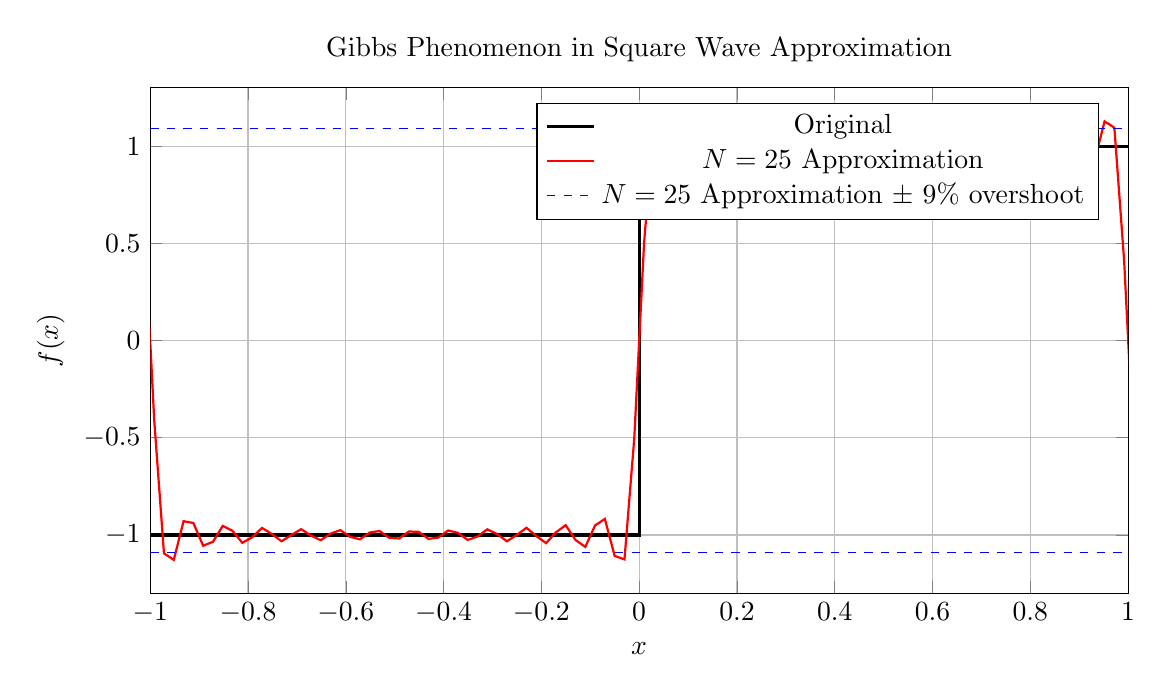
\begin{tikzpicture}
        \begin{axis}[
                width=14cm, height=8cm,
                xlabel={\(x\)},
                ylabel={\(f(x)\)},
                title={Gibbs Phenomenon in Square Wave Approximation},
                xmin=-1, xmax=1,
                ymin=-1.3, ymax=1.3,
                grid=major,
                legend pos=north east,
                samples=500
            ]

            % Original square wave around discontinuity
            \addplot[black, very thick, const plot] coordinates {
                    (-1, -1) (0, -1) (0, 1) (1, 1)
                };
            \addlegendentry{Original}

            % High-order approximation showing Gibbs phenomenon
            \addplot[red, thick] {(4/pi)*(sin(deg(pi*x)) + sin(deg(3*pi*x))/3 + sin(deg(5*pi*x))/5 + sin(deg(7*pi*x))/7 + sin(deg(9*pi*x))/9 + sin(deg(11*pi*x))/11 + sin(deg(13*pi*x))/13 + sin(deg(15*pi*x))/15 + sin(deg(17*pi*x))/17 + sin(deg(19*pi*x))/19 + sin(deg(21*pi*x))/21 + sin(deg(23*pi*x))/23 + sin(deg(25*pi*x))/25)};
            \addlegendentry{\(N=25\) Approximation}

            % Show the 9% overshoot lines
            \addplot[blue, dashed] coordinates {(-1, 1.09) (1, 1.09)};
            \addplot[blue, dashed] coordinates {(-1, -1.09) (1, -1.09)};
            \addlegendentry{\(N=25\) Approximation \(\pm\) 9\% overshoot}

        \end{axis}
    \end{tikzpicture}
    \end{document}